\begin{figure}[ht]
  \centering
  \begin{subfigure}{0.14\linewidth}
 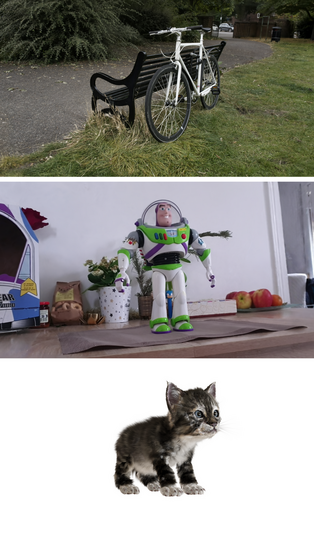
\includegraphics[width=\linewidth]{images/composition/buzz_riding_cat/scenes.png}
 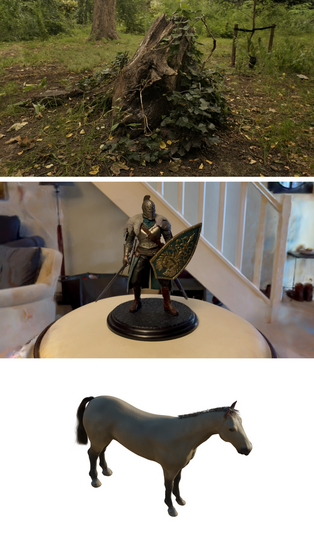
\includegraphics[width=\linewidth]{images/composition/knight_and_horse/scenes.png}
 \caption{Scenes}
  \end{subfigure}
  %
  \hfill
  %
  \begin{subfigure}{0.42\linewidth}
 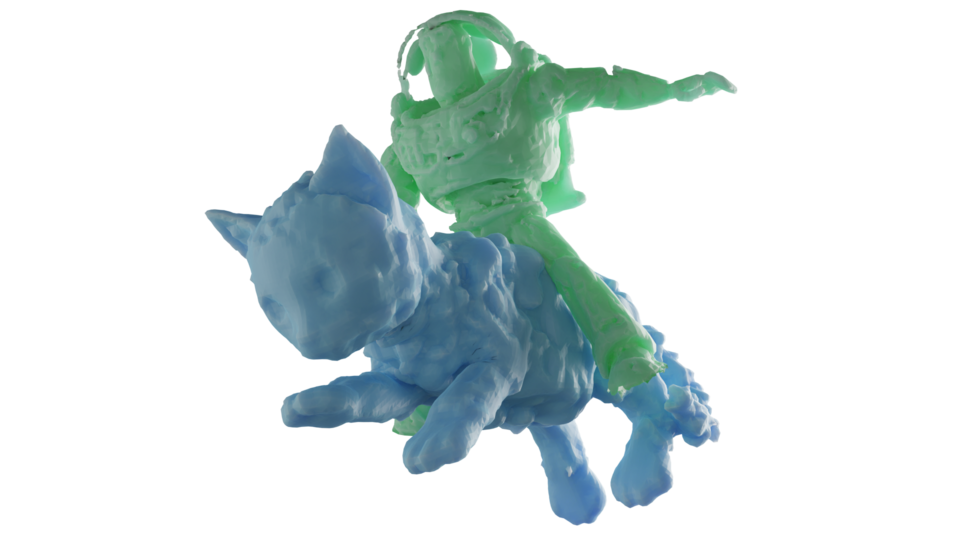
\includegraphics[width=\linewidth]{images/composition/buzz_riding_cat/mesh.png}
 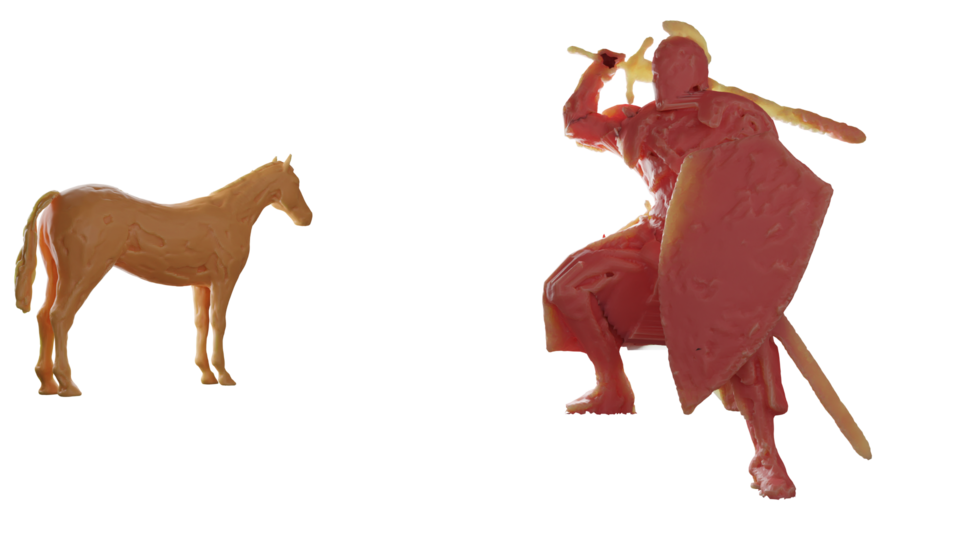
\includegraphics[width=\linewidth]{images/composition/knight_and_horse/mesh.png}
  \caption{Posing foreground meshes}
  \end{subfigure}
  %
  \hfill
  \begin{subfigure}{0.42\linewidth}
 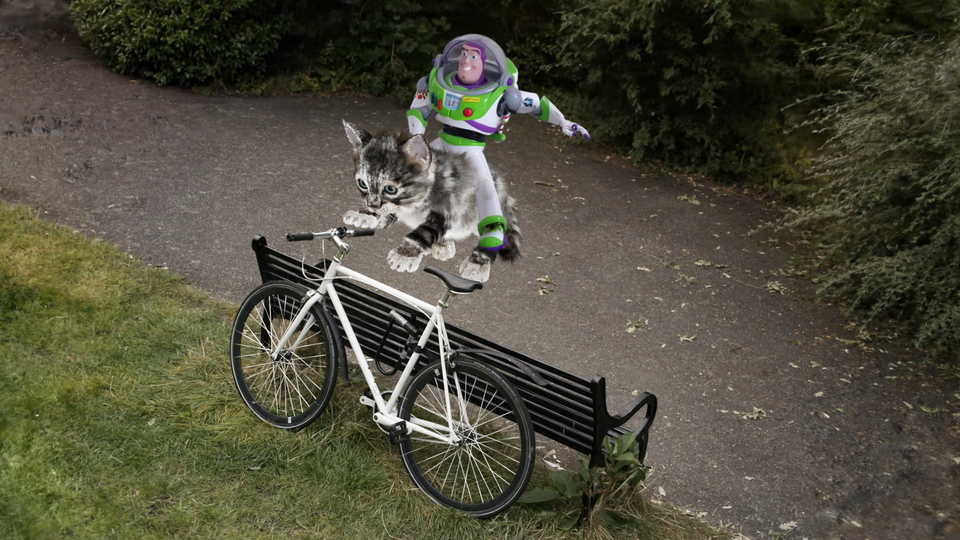
\includegraphics[width=\linewidth]{images/composition/buzz_riding_cat/0_0.png}
 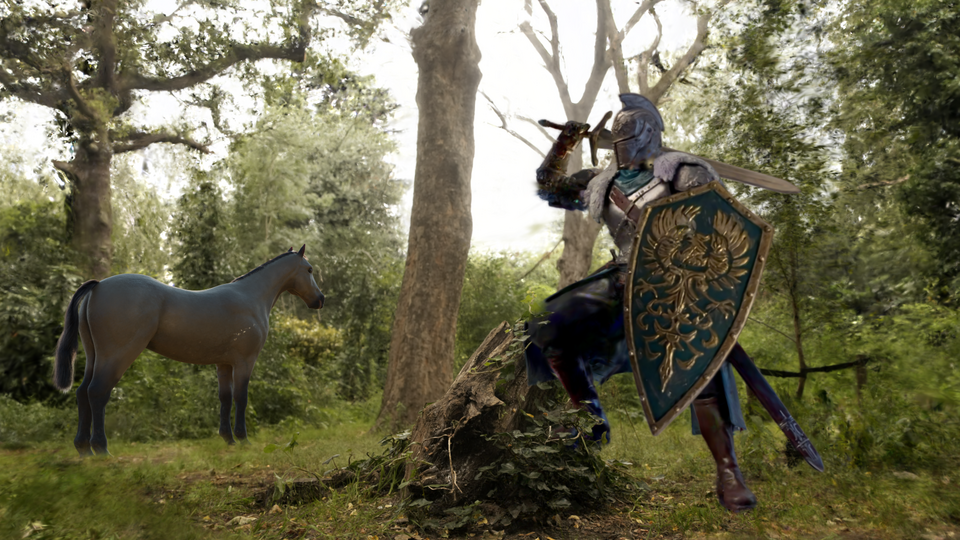
\includegraphics[width=\linewidth]{images/composition/knight_and_horse/0_1.png}
  \caption{Rendering composition}
  \end{subfigure}
  %
  \caption{
  \textbf{Scene composition.} Using mesh editing tools in Blender, we were able to combine various elements from multiple scenes (a) to build a whole new scene (c). We also changed the pose of the characters by using the rigging tool in Blender (b). Similarly to surface-based methods like SuGaR~\cite{guedon2023sugar}, Frosting can be used for editing and compositing scenes, but allows for better rendering of complex volumetric effects and fuzzy materials, such as hair or grass.
  }
  \label{fig:scene-composition}
\end{figure}

\section{Related Work}

The goal of image-based rendering (IBR) is to create a representation of a scene from a given set of images in order to generate new images of the scene. Different types of scene representations have been proposed, ranging from explicit and editable ones like triangle meshes or point clouds, to implicit or non-editable ones like voxel grids, multiplane images, or neural implicit functions. 

\noindent
\textbf{Volumetric IBR methods.} A recent breakthrough in IBR is Neural Radiance Fields (NeRF)~\cite{mildenhall2020nerf}, which uses a multilayer perceptron (MLP) to model a continuous volumetric function of density and color. NeRF can render novel views with high quality and view-dependent effects, by using volumetric ray tracing. However, NeRF is slow and memory hungry. 
%
Several works have tried to improve NeRF’s efficiency and training speed by using discretized volumetric representations like voxel grids and hash tables to store learnable features that act as inputs for a much smaller MLP~\cite{chen-eccv-2022-tensorf, karnewar2022relu, mueller2022instantngp, sun2022direct, yu_and_fridovichkeil2021plenoxels}, or to improve rendering performance by using hierarchical sampling strategies~\cite{barron2022mipnerf360,hedman2021snerg,reiser2021kilonerf,yu2021plenoctrees}. Other works have also proposed to modify NeRF's representation of radiance and include an explicit lighting model to increase the rendering quality for scenes with specular materials~\cite{verbin2022ref, boss2021nerd, kuang2022neroic, srinivasan2021nerv, zhang2021physg}. 
%
However, most volumetric methods rely on implicit representations that are not suited to editing compared to triangle meshes, for which most standard graphics hardware and software are tailored.

\noindent
\textbf{Surface-based IBR methods.} Triangle meshes have been a popular 3D representation for generating novel views of scenes~\cite{wood:2000:slf,buehler2001unstructured,hedman-2018-deepblending} after Structure-from-motion (SfM)~\cite{snavely-2006-structure-from-motion} and multi-view stereo (MVS)~\cite{goesele-2007-multiviewstereo} have enabled 3D reconstruction of surfaces. 
%
Deep-learning-based mesh representations~\cite{riegler2020free,riegler2021stable} have also been used for improving view synthesis using explicit surface meshes; However, even though mesh-based methods allow for very efficient rendering, they have trouble capturing complex and very fine geometry as well as fuzzy materials.

\noindent
\textbf{Hybrid IBR methods.} Some methods use a hybrid volumetric representation to recover surface meshes that are suitable for downstream graphics applications while efficiently modeling view-dependent appearance. 
%
Specifically, some works optimize a Neural Radiance Field in which the density is replaced by an implicit signed distance function (SDF), which provides a stronger regularization on the underlying geometry~\cite{oechsle2021unisurf,yariv2021volsdf,wang2021neus,li-cvpr2023-neuralangelo,darmon-2022-warp,bao-2022-neumesh}. However, most of these methods are not aimed at real-time rendering.
To mitigate this issue, other approaches greatly accelerate rendering by ``baking'' the rendering computation into the extracted mesh after optimization with a dedicated view-dependent appearance model~\cite{chen2022mobilenerf,yariv-2023-bakedsdf,reiser2024binaryopacitygrid}. 
%
Even though these surface-based methods encode the surface using a volumetric function represented by an MLP during optimization, they struggle in capturing fine details or fuzzy materials compared to volumetric methods.

Adaptive Shells~\cite{wang-siggraphasia2023-adaptive-shells} is a recent method that achieves a significant improvement in rendering quality by using a true hybrid surface-volumetric approach that restricts the volumetric rendering of NeRFs to a thin layer around the object. This layer is bounded by two explicit meshes, which are extracted after optimizing an SDF-based radiance field. The layer’s variable thickness also improves the rendering quality compared to a single flat mesh. This method combines the high-quality rendering of a full volumetric approach with the editability of a surface-based approach by manipulating the two meshes that define the layer. However, Adaptive Shells depends on a neural SDF~\cite{wang2021neus}, which has some limitations in its ability to reconstruct precise surfaces, and requires more than 8 hours to optimize a single synthetic scene, which is much longer than the recent Gaussian Splatting methods. 

\noindent
\textbf{Gaussian Splatting.} Gaussian Splatting~\cite{kerbl3Dgaussians} is a new volumetric representation inspired by point cloud-based radiance fields~\cite{kopanas2021point, ruckert2021adop} which is very fast to optimize and allows for real-time rendering with very good quality. One of its greatest strengths is its explicit 3D representation, which enables editing tasks as each Gaussian exists individually and can be easily adjusted in real-time. 
%
Some appearance editing and segmentation methods have been proposed~\cite{chen2023gaussianeditor,huang2023pointn,chungmin-2024-garfield,ye-2023-gaussian_grouping}, but the lack of structure in the point cloud makes it almost impossible for a 3D artist or an animator to easily modify, sculpt or animate the raw representation. The triangle mesh remains the standard 3D structure for these applications.
%
A recent work, SuGaR~\cite{guedon2023sugar}, extends this framework by aligning the Gaussians with the surface and extracting a mesh from them. Gaussians are finally flattened and pinned on the surface of the mesh, which provides a hybrid representation combining the editability of a mesh with the high-quality rendering of Gaussian Splatting. However, SuGaR remains a surface-based representation with limited capacity in reconstructing and rendering fuzzy materials and volumetric effects, resulting in a decrease in performance compared to vanilla Gaussian Splatting.